\subsection*{Problema 15}

\textbf{Enunciado:} Calcular la integral:
\begin{equation*}
\int \frac{(1 - \sin x) \, dx}{(1 + \sin x)\sin x}
\end{equation*}

\textbf{Solución:} 
Para resolver la integral dada, empleamos la sustitución universal del semiénculo, también conocida como sustitución de Weierstrass. Definimos la variable auxiliar:
\begin{equation*}
z = \tan\left(\frac{x}{2}\right)
\end{equation*}

De esta definición, las funciones trigonométricas y el diferencial se expresan en términos de $z$ de la siguiente manera:
\begin{align*}
\sin x &= \frac{2z}{1 + z^2}, \quad 
\cos x = \frac{1 - z^2}{1 + z^2}, \\
dx &= \frac{2 \, dz}{1 + z^2}
\end{align*}

Sustituimos estas expresiones en la integral original. Primero, simplificamos el denominador y el numerador en función de $z$:
\begin{align*}
1 + \sin x &= 1 + \frac{2z}{1 + z^2} = \frac{1 + z^2 + 2z}{1 + z^2} \\
&= \frac{(1 + z)^2}{1 + z^2}
\end{align*}

Ahora, sustituimos los componentes en la integral:
\begin{align*}
\int &\frac{\left(1 - \frac{2z}{1 + z^2}\right) \frac{2 \, dz}{1 + z^2}}{\left(\frac{(1 + z)^2}{1 + z^2}\right)\left(\frac{2z}{1 + z^2}\right)} \\
&= \int \frac{\left(\frac{1 + z^2 - 2z}{1 + z^2}\right)}{\frac{2z(1 + z)^2}{(1 + z^2)^2}} \cdot \frac{2 \, dz}{1 + z^2}
\end{align*}

Simplificando los términos comunes y el factor $2$, la expresión se reduce a:
\begin{align*}
&= \int \frac{(z - 1)^2 (1 + z^2)}{z(1 + z)^2 (1 + z^2)} \, dz \\
&= \int \frac{(z - 1)^2}{z(z + 1)^2} \, dz
\end{align*}

Desarrollamos el binomio en el numerador:
\begin{equation*}
\int \frac{z^2 - 2z + 1}{z(z + 1)^2} \, dz
\end{equation*}

Aplicamos el método de descomposición en fracciones parciales para el integrando racional:
\begin{equation*}
\frac{z^2 - 2z + 1}{z(z + 1)^2} = \frac{A}{z} + \frac{B}{z + 1} + \frac{C}{(z + 1)^2}
\end{equation*}

Multiplicamos toda la ecuación por el denominador común $z(z + 1)^2$:
\begin{multline*}
z^2 - 2z + 1 = A(z + 1)^2 \\
+ Bz(z + 1) + Cz
\end{multline*}

Para hallar las constantes, evaluamos en valores convenientes de $z$:
\begin{itemize}
    \item Si $z = 0$: $1 = A(1)^2 \implies A = 1$.
    \item Si $z = -1$: 
    \begin{equation*}
    (-1)^2 - 2(-1) + 1 = C(-1) \implies 4 = -C \implies C = -4
    \end{equation*}
    \item Coeficientes de $z^2$: $1 = A + B \implies B = 1 - 1 = 0$.
\end{itemize}

Sustituimos los valores de $A$, $B$ y $C$ en la descomposición:
\begin{equation*}
\int \left( \frac{1}{z} - \frac{4}{(z + 1)^2} \right) dz
\end{equation*}

Integramos cada término por separado:
\begin{align*}
\int \frac{1}{z} \, dz &= \ln|z| \\
\int \frac{-4}{(z + 1)^2} \, dz &= \frac{4}{z + 1}
\end{align*}

Juntando los resultados parciales e incorporando la constante de integración $C_1$:
\begin{equation*}
\ln|z| + \frac{4}{z + 1} + C_1
\end{equation*}

Finalmente, regresamos a la variable original $x$ sustituyendo $z = \tan(x/2)$:
\begin{equation*}
\ln\left|\tan\left(\frac{x}{2}\right)\right| + \frac{4}{\tan\left(\frac{x}{2}\right) + 1} + C
\end{equation*}

\begin{figure}[H]
	\centering
	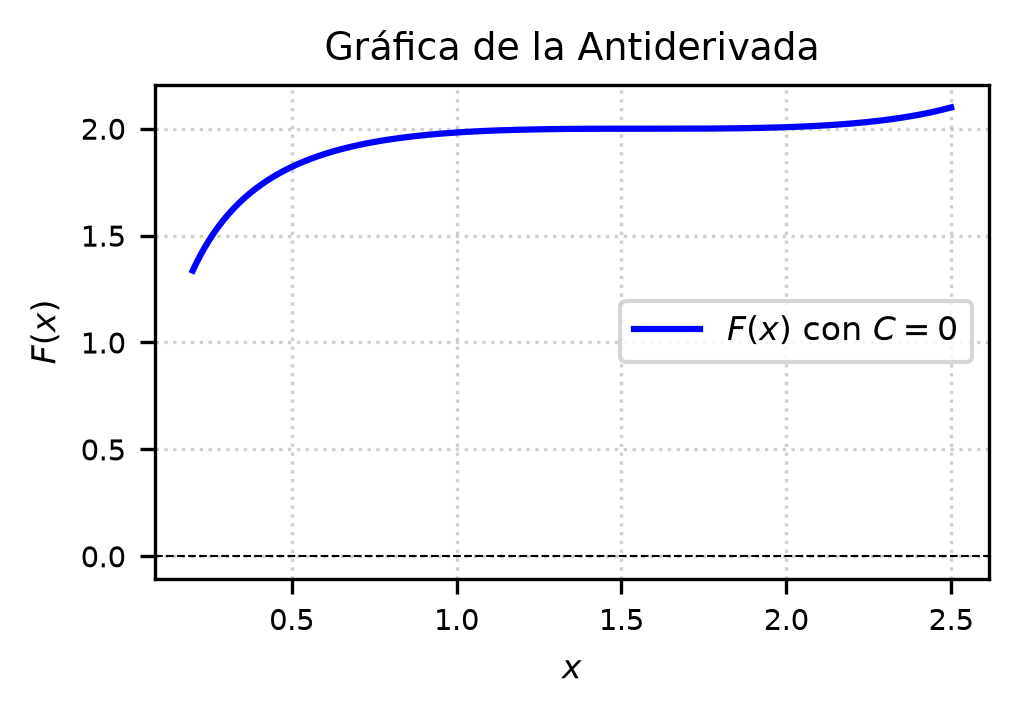
\includegraphics[width=\columnwidth]{semana_04/graficas/SEM04_P15_grafica.png}
	\caption{Representación gráfica de $f(x)$ y su antiderivada $F(x)$ evaluada para la constante de integración $C = 0$ (Problema 15).}
	\label{fig:problema15}
\end{figure}
